\documentclass[border=4pt]{standalone}
\usepackage{amsmath,amssymb}
\usepackage{tikz}
\usetikzlibrary{arrows.meta}
\begin{document}
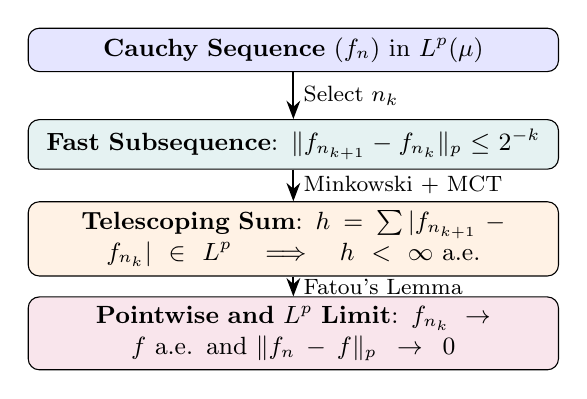
\begin{tikzpicture}[font=\small, >=Stealth]
  \node[draw, rounded corners, fill=blue!10, text width=6.5cm, align=center] (C1) at (0, 3.6)
    {\textbf{Cauchy Sequence} $(f_n)$ in $L^p(\mu)$};
  \node[draw, rounded corners, fill=teal!10, text width=6.5cm, align=center] (C2) at (0, 2.4)
    {\textbf{Fast Subsequence}: $\|f_{n_{k+1}} - f_{n_k}\|_p \le 2^{-k}$};
  \node[draw, rounded corners, fill=orange!10, text width=6.5cm, align=center] (C3) at (0, 1.2)
    {\textbf{Telescoping Sum}: $h = \sum |f_{n_{k+1}} - f_{n_k}| \in L^p \implies h < \infty$ a.e.};
  \node[draw, rounded corners, fill=purple!10, text width=6.5cm, align=center] (C4) at (0, 0.0)
    {\textbf{Pointwise and $L^p$ Limit}: $f_{n_k} \to f$ a.e. and $\|f_n - f\|_p \to 0$};

  \draw[->, thick] (C1) -- node[right, font=\footnotesize] {Select $n_k$} (C2);
  \draw[->, thick] (C2) -- node[right, font=\footnotesize] {Minkowski + MCT} (C3);
  \draw[->, thick] (C3) -- node[right, font=\footnotesize] {Fatou's Lemma} (C4);
\end{tikzpicture}
\end{document}